\documentclass[conference]{IEEEtran}

\usepackage[T1]{fontenc}
\usepackage{cite}
\usepackage{amsmath,amssymb,amsfonts}
\usepackage{booktabs}
\usepackage{multirow}
\usepackage{array}
\usepackage{graphicx}
\usepackage{xcolor}
\usepackage{url}
\usepackage{tikz}
\usepackage{pgfplots}
\usepackage{siunitx}
\usepackage{enumitem}
\usepackage{balance}

\pgfplotsset{compat=1.18}
\usetikzlibrary{arrows.meta,positioning,shapes.geometric,fit,backgrounds}

\title{Multi-Agent Framework for Uncertainty-Aware Resource Allocation and Auto-Scaling in Distributed Systems}

\author{
\IEEEauthorblockN{Your Name}
\IEEEauthorblockA{
Department / Institution\\
City, Country\\
email@example.com}
\and
\IEEEauthorblockN{Co-Author Name}
\IEEEauthorblockA{
Department / Institution\\
City, Country\\
email@example.com}
}

\begin{document}

\maketitle

\begin{abstract}
Auto-scaling remains a central systems problem because controllers must react to changing demand without causing instability, excessive resource consumption, or delayed service response. Threshold-based and purely reactive strategies are attractive because they are simple, but they may fail to account for uncertainty in future workload conditions. This paper presents a microservice-based research prototype for uncertainty-aware resource allocation and auto-scaling in distributed systems. The framework combines node-level metric simulation, workload generation, lightweight sequence forecasting, uncertainty-aware risk scoring, multi-agent evaluation, resource planning, policy-based decision making, action execution, and evaluation into a reproducible experimental pipeline. The implementation is containerized, instrumented for observability, and supported by a deterministic experiment runner with provenance capture, batch reporting, confidence intervals, pairwise comparisons, and paper-ready output artifacts. The strongest validated batch contains 30 runs across three policies over 20 timesteps per run. Results show that the proposed uncertainty-aware policy yields the lowest mean risk among the evaluated policies while exhibiting substantially more adaptive action behavior than threshold and reactive baselines. These findings position the framework as a strong research prototype for controlled experimentation on uncertainty-aware scaling.
\end{abstract}

\begin{IEEEkeywords}
distributed systems, auto-scaling, resource allocation, multi-agent systems, uncertainty-aware control, reproducible experiments, microservices
\end{IEEEkeywords}

\section{Introduction}
Distributed systems operate under changing and often imperfectly observable workload conditions. A practical auto-scaling controller must decide whether to increase, decrease, or hold resources while balancing efficiency, stability, and responsiveness. Conventional rule-based policies often work well in stable conditions, yet they can become brittle under noisy, bursty, or rapidly shifting workloads because they reason almost entirely about the current state.

This paper explores an uncertainty-aware alternative implemented as a modular microservice framework. Instead of mapping a single utilization signal directly to a control action, the framework combines prediction, uncertainty estimation, risk scoring, multi-agent evaluation, and resource planning before producing a scaling decision. The goal is not to claim a production-grade controller, but to build a credible and reproducible research platform for comparing decision policies under controlled conditions.

The paper asks the following research question:
\begin{quote}
How does an uncertainty-aware multi-agent auto-scaling policy behave relative to threshold-based and reactive baselines in a controlled distributed-system simulation?
\end{quote}

The main contributions of this work are:
\begin{enumerate}[leftmargin=*]
\item A complete microservice architecture for uncertainty-aware scaling experiments.
\item A deterministic and auditable experiment workflow with run provenance, trace control, and repeated batch execution.
\item A comparative empirical evaluation of proposed, threshold, and reactive policies with confidence intervals and pairwise reporting.
\item IEEE-ready tables and diagrams derived from the implemented framework and validated result bundles.
\end{enumerate}
These contributions align with prior systems work on cluster-scale resource orchestration and tail-sensitive performance in distributed infrastructure \cite{borg2015,autopilot2020,borgomega2016,tail2013}.

\section{Problem Formulation}
Auto-scaling can be framed as a sequential control problem. At time step $t$, the framework observes system state
\[
S_t = \{u_t^{cpu}, u_t^{mem}, w_t, h_t\},
\]
where $u_t^{cpu}$ and $u_t^{mem}$ are node utilization signals, $w_t$ is the current workload, and $h_t$ is the recent workload history. The controller produces a one-step demand estimate $\hat{w}_{t+1}$ and an uncertainty score $\sigma_t$, then derives a normalized risk signal $r_t \in [0,1]$ and selects an action
\[
a_t \in \{\texttt{scale\_up}, \texttt{hold}, \texttt{scale\_down}\}.
\]

The objective is not merely to minimize immediate error, but to favor decisions that remain stable and interpretable while responding to uncertain demand. This motivates the use of an uncertainty-aware intermediate representation rather than a direct threshold on current load.

\section{System Architecture}
The framework is organized as a set of FastAPI microservices, each responsible for one stage of the sensing, decision, execution, or evaluation pipeline. This decomposition makes the system easy to observe, reset, replace, and extend during experiments.

\begin{figure}[!t]
\centering
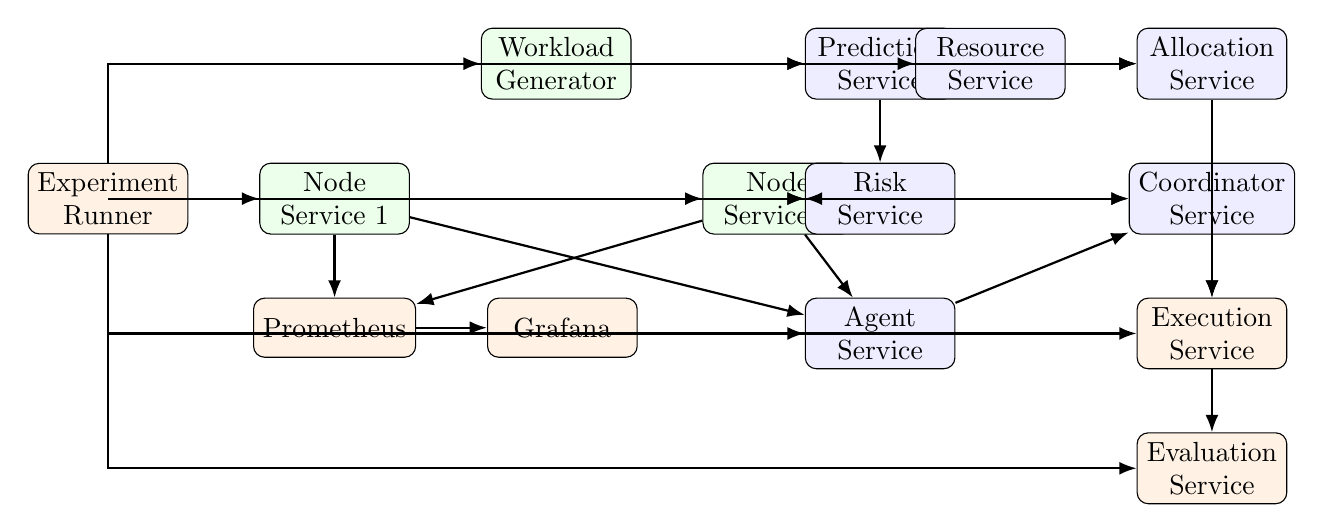
\begin{tikzpicture}[
node distance=0.8cm and 0.9cm,
service/.style={draw, rounded corners, align=center, minimum width=1.9cm, minimum height=0.75cm, fill=blue!7},
obs/.style={draw, rounded corners, align=center, minimum width=1.9cm, minimum height=0.75cm, fill=green!8},
eval/.style={draw, rounded corners, align=center, minimum width=1.9cm, minimum height=0.75cm, fill=orange!10},
arrow/.style={-{Latex[length=2.2mm]}, thick}
]
\node[obs] (wg) {Workload\\Generator};
\node[obs, below left=of wg] (ns1) {Node\\Service 1};
\node[obs, below right=of wg] (ns2) {Node\\Service 2};

\node[service, right=2.2cm of wg] (pred) {Prediction\\Service};
\node[service, below=of pred] (risk) {Risk\\Service};
\node[service, below=of risk] (agent) {Agent\\Service};
\node[service, right=2.2cm of risk] (coord) {Coordinator\\Service};
\node[service, above=of coord] (alloc) {Allocation\\Service};
\node[service, left=of alloc] (res) {Resource\\Service};
\node[eval, below=of coord] (exec) {Execution\\Service};
\node[eval, below=of exec] (metric) {Evaluation\\Service};
\node[eval, below=of ns1] (prom) {Prometheus};
\node[eval, right=of prom] (graf) {Grafana};
\node[eval, left=of ns1] (exp) {Experiment\\Runner};

\draw[arrow] (wg) -- (pred);
\draw[arrow] (pred) -- (risk);
\draw[arrow] (ns1) -- (risk);
\draw[arrow] (ns2) -- (risk);
\draw[arrow] (ns1) -- (agent);
\draw[arrow] (ns2) -- (agent);
\draw[arrow] (risk) -- (coord);
\draw[arrow] (agent) -- (coord);
\draw[arrow] (pred) |- (alloc);
\draw[arrow] (res) -- (alloc);
\draw[arrow] (coord) -- (exec);
\draw[arrow] (alloc) -- (exec);
\draw[arrow] (exec) -- (metric);
\draw[arrow] (ns1) -- (prom);
\draw[arrow] (ns2) -- (prom);
\draw[arrow] (prom) -- (graf);

\draw[arrow] (exp) |- (wg);
\draw[arrow] (exp) -- (ns1);
\draw[arrow] (exp) |- (ns2);
\draw[arrow] (exp) |- (pred);
\draw[arrow] (exp) |- (risk);
\draw[arrow] (exp) |- (agent);
\draw[arrow] (exp) |- (res);
\draw[arrow] (exp) |- (alloc);
\draw[arrow] (exp) |- (coord);
\draw[arrow] (exp) |- (exec);
\draw[arrow] (exp) |- (metric);
\end{tikzpicture}
\caption{Microservice architecture of the proposed uncertainty-aware scaling framework.}
\label{fig:architecture}
\end{figure}

Table~\ref{tab:services} summarizes the major services used in the framework.

\begin{table}[!t]
\caption{Framework services and primary outputs}
\label{tab:services}
\centering
\footnotesize
\begin{tabular}{p{2.2cm} p{4.2cm} p{1.6cm}}
\toprule
\textbf{Service} & \textbf{Role} & \textbf{Output} \\
\midrule
Node service & Simulates node-level CPU and memory signals & \texttt{/metrics} \\
Workload generator & Produces dynamic workload input & \texttt{/load} \\
Prediction service & Returns next-step prediction and uncertainty & \texttt{/predict} \\
Risk service & Computes normalized instability risk & \texttt{/risk} \\
Agent service & Produces performance, cost, and risk scores & \texttt{/evaluate} \\
Resource service & Tracks available simulated resources & \texttt{/resources} \\
Allocation service & Builds greedy resource plans & \texttt{/allocate} \\
Coordinator service & Emits logical scaling decisions & \texttt{/decide} \\
Execution service & Applies simulated actions and tracks history & \texttt{/execute} \\
Evaluation service & Maintains RMSE and utilization metrics & \texttt{/metrics} \\
\bottomrule
\end{tabular}
\end{table}

\section{Methodology}
\subsection{Signal Flow and Decision Stages}
Each timestep consists of the following sequence:
\begin{enumerate}[leftmargin=*]
\item Collect node CPU and memory observations.
\item Acquire workload and produce the effective workload trace.
\item Forecast next-step load and uncertainty.
\item Compute a normalized risk score from utilization and uncertainty.
\item Evaluate agent-level perspectives on performance, cost, and risk.
\item Inspect resources and compute a feasible allocation plan.
\item Select an action according to the active policy.
\item Execute the action and log resulting metrics.
\end{enumerate}

\begin{figure}[!t]
\centering
\begin{tikzpicture}[
node distance=0.55cm and 0.45cm,
step/.style={draw, rounded corners, align=center, minimum width=2.2cm, minimum height=0.7cm, fill=gray!9},
arrow/.style={-{Latex[length=2mm]}, thick}
]
\node[step] (a) {Load config};
\node[step, below=of a] (b) {Reset services};
\node[step, below=of b] (c) {Wait readiness};
\node[step, below=of c] (d) {Collect metrics};
\node[step, below=of d] (e) {Predict \& estimate uncertainty};
\node[step, below=of e] (f) {Compute risk};
\node[step, below=of f] (g) {Evaluate agents};
\node[step, below=of g] (h) {Plan allocation};
\node[step, below=of h] (i) {Select policy action};
\node[step, below=of i] (j) {Execute action};
\node[step, below=of j] (k) {Record evaluation};
\node[step, below=of k] (l) {Persist artifacts};

\foreach \x/\y in {a/b,b/c,c/d,d/e,e/f,f/g,g/h,h/i,i/j,j/k,k/l}
    \draw[arrow] (\x) -- (\y);
\end{tikzpicture}
\caption{Experiment workflow used for repeated policy and scenario evaluations.}
\label{fig:workflow}
\end{figure}

\subsection{Prediction and Risk Modeling}
The prediction service uses a lightweight recurrent-style model that extracts a level term, a momentum term, a volatility term, and a hidden-state trend adjustment from recent history. This choice avoids heavyweight dependencies while preserving trend-aware behavior. The resulting uncertainty score is derived from volatility and absolute momentum, producing higher uncertainty under noisier or more rapidly changing inputs.

The risk service combines utilization and uncertainty through the following normalized heuristic:
\begin{equation}
r_t = 0.55\bar{u}_t + 0.25\sigma_t + 1.2\,\mathrm{Var}(u_t^{cpu},u_t^{mem},\sigma_t) + 0.10|u_t^{cpu} - u_t^{mem}|,
\label{eq:risk}
\end{equation}
where $\bar{u}_t = (u_t^{cpu} + u_t^{mem}) / 2$. This design emphasizes current pressure while preserving sensitivity to instability and imbalance.

\subsection{Multi-Agent Evaluation}
The agent layer computes three interpretable scores:
\begin{align}
s_t^{perf} &= 0.85\,u_t^{cpu} + 0.15(1-r_t), \\
s_t^{cost} &= 0.70(1-u_t^{cpu}) + 0.30(1-r_t), \\
s_t^{risk} &= r_t.
\end{align}
These scores do not represent independent learning agents; rather, they encode multiple perspectives that can be logged and analyzed consistently across runs.

\subsection{Policies}
Three policies are compared:
\begin{itemize}[leftmargin=*]
\item \textbf{Proposed}: Uses prediction and risk jointly. It scales up when $\hat{w}_{t+1} \geq 0.6$ and $r_t \geq 0.4$, scales down when $\hat{w}_{t+1} \leq 0.35$ and $r_t \leq 0.4$, and otherwise holds.
\item \textbf{Threshold}: Uses direct CPU and workload thresholds without explicit uncertainty modeling.
\item \textbf{Reactive}: Uses recent workload change and current CPU utilization.
\end{itemize}

\subsection{Experimental Setup}
The strongest validated batch in the repository contains:
\begin{itemize}[leftmargin=*]
\item 10 runs for each policy,
\item 20 timesteps per run,
\item 30 total runs,
\item deterministic generated traces for repeatability,
\item per-run configuration, workload trace, summary, log, and provenance artifacts.
\end{itemize}

The framework supports Docker-based deployment, automatic state reset between runs, service readiness checks, confidence interval reporting, and pairwise comparison bundles. This combination is intended to make experimental claims inspectable and repeatable.
To strengthen inferential rigor, pairwise comparisons are reported with permutation tests, bootstrap confidence intervals, Cliff's delta effect sizes, and Holm-Bonferroni corrected p-values.

\section{Results}
Table~\ref{tab:policy-results} presents the main policy-comparison batch. The proposed policy achieves the lowest mean risk and is the only policy that consistently exhibits both scale-up and scale-down behavior across repeated runs.

\begin{table*}[!t]
\caption{Policy comparison over 30 total runs (10 per policy)}
\label{tab:policy-results}
\centering
\footnotesize
\begin{tabular}{lccccccc}
\toprule
\textbf{Policy} & \textbf{Runs} & \textbf{Success Rate} & \textbf{RMSE} & \textbf{Utilization} & \textbf{Prediction} & \textbf{Risk} & \textbf{Action Distribution} \\
\midrule
Proposed & 10 & 100.0\% & 0.058 $\pm$ 0.014 & 0.5976 $\pm$ 0.0438 & 0.5367 $\pm$ 0.0892 & 0.3791 $\pm$ 0.0354 & hold: 170, up: 24, down: 6 \\
Threshold & 10 & 100.0\% & 0.053 $\pm$ 0.0095 & 0.5990 $\pm$ 0.0384 & 0.5398 $\pm$ 0.1211 & 0.3817 $\pm$ 0.0280 & hold: 199, up: 1, down: 0 \\
Reactive & 10 & 100.0\% & 0.061 $\pm$ 0.0160 & 0.6065 $\pm$ 0.0452 & 0.5131 $\pm$ 0.1387 & 0.3870 $\pm$ 0.0331 & hold: 200, up: 0, down: 0 \\
\bottomrule
\end{tabular}
\end{table*}

\begin{figure}[!t]
\centering
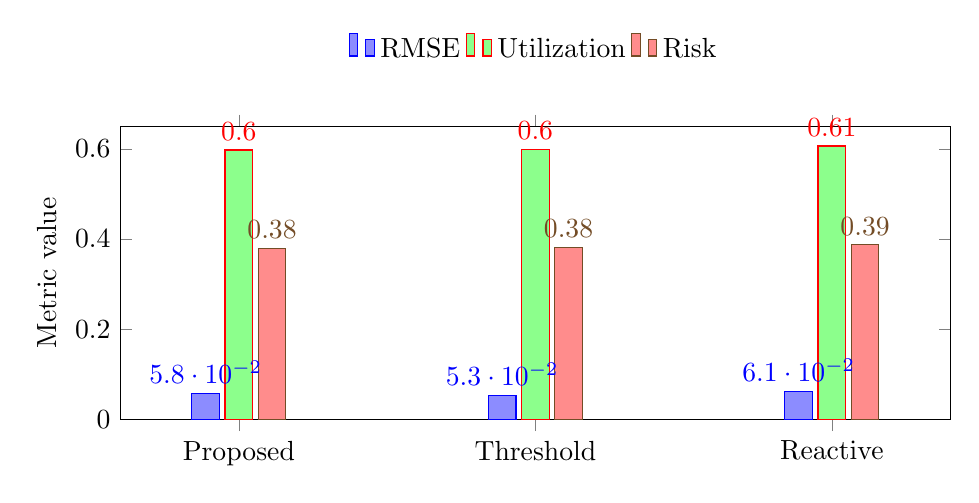
\begin{tikzpicture}
\begin{axis}[
    width=\columnwidth,
    height=5.3cm,
    ybar,
    bar width=10pt,
    ymin=0,
    ymax=0.65,
    symbolic x coords={Proposed,Threshold,Reactive},
    xtick=data,
    ylabel={Metric value},
    legend style={at={(0.5,1.18)}, anchor=south, legend columns=3, draw=none},
    nodes near coords,
    nodes near coords align={vertical},
    enlarge x limits=0.20
]
\addplot+[fill=blue!45] coordinates {(Proposed,0.058) (Threshold,0.053) (Reactive,0.061)};
\addplot+[fill=green!45] coordinates {(Proposed,0.5976) (Threshold,0.5990) (Reactive,0.6065)};
\addplot+[fill=red!45] coordinates {(Proposed,0.3791) (Threshold,0.3817) (Reactive,0.3870)};
\legend{RMSE,Utilization,Risk}
\end{axis}
\end{tikzpicture}
\caption{Main policy comparison using the mean values of RMSE, utilization, and risk.}
\label{fig:policy-bars}
\end{figure}

\begin{figure}[!t]
\centering
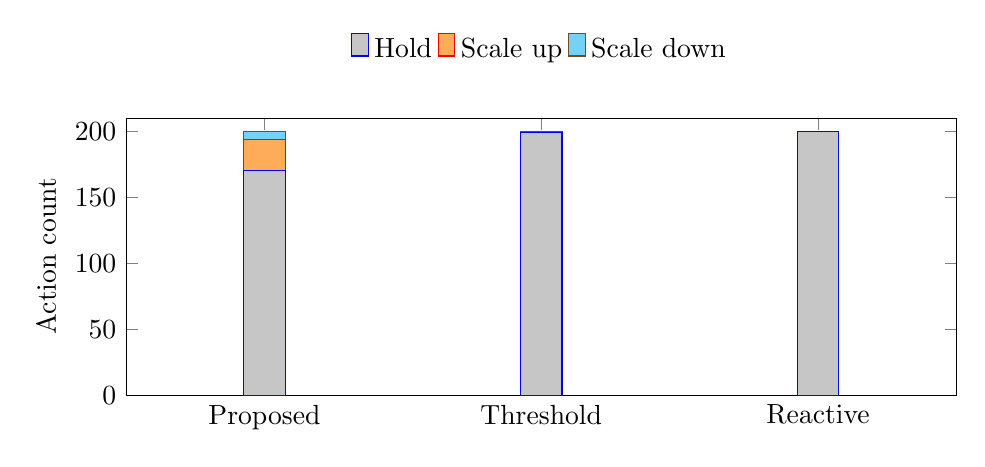
\begin{tikzpicture}
\begin{axis}[
    width=\columnwidth,
    height=5.1cm,
    ybar stacked,
    bar width=15pt,
    ymin=0,
    ymax=210,
    symbolic x coords={Proposed,Threshold,Reactive},
    xtick=data,
    ylabel={Action count},
    legend style={at={(0.5,1.16)}, anchor=south, legend columns=3, draw=none},
    enlarge x limits=0.25
]
\addplot+[fill=gray!45] coordinates {(Proposed,170) (Threshold,199) (Reactive,200)};
\addplot+[fill=orange!65] coordinates {(Proposed,24) (Threshold,1) (Reactive,0)};
\addplot+[fill=cyan!55] coordinates {(Proposed,6) (Threshold,0) (Reactive,0)};
\legend{Hold,Scale up,Scale down}
\end{axis}
\end{tikzpicture}
\caption{Action distribution across the 200 actions produced by each policy over repeated runs.}
\label{fig:action-stacked}
\end{figure}

To complement policy comparison, Table~\ref{tab:scenario-results} summarizes scenario-level behavior under baseline, bursty, and mixed workload regimes. Bursty conditions produce the highest prediction and utilization, while the mixed workload regime pushes the controller toward lower predicted demand and more frequent scale-down behavior.

\begin{table}[!t]
\caption{Scenario comparison reference batch}
\label{tab:scenario-results}
\centering
\footnotesize
\begin{tabular}{lccccc}
\toprule
\textbf{Scenario} & \textbf{Runs} & \textbf{RMSE} & \textbf{Utilization} & \textbf{Prediction} & \textbf{Risk} \\
\midrule
Baseline & 3 & 0.0667 & 0.6600 & 0.5847 & 0.3787 \\
Bursty & 3 & 0.1100 & 0.7111 & 0.7989 & 0.4556 \\
Mixed & 3 & 0.1067 & 0.6607 & 0.2613 & 0.3847 \\
\bottomrule
\end{tabular}
\end{table}

\begin{figure}[!t]
\centering
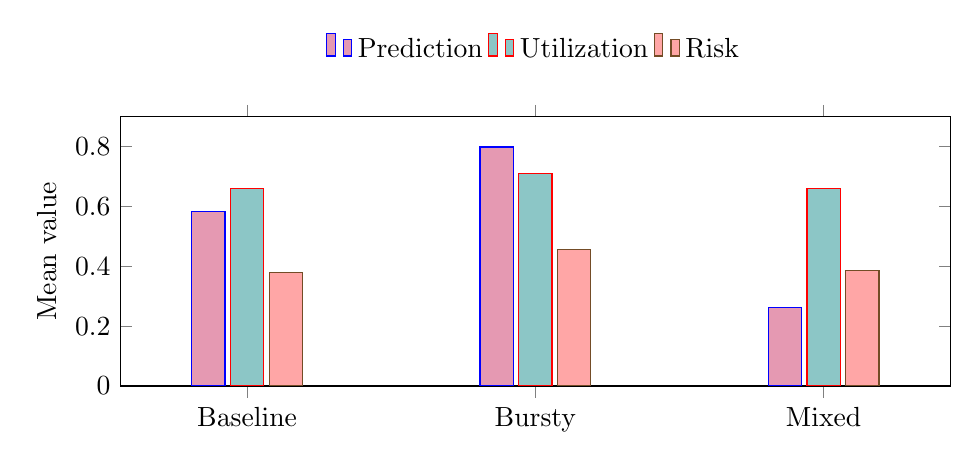
\begin{tikzpicture}
\begin{axis}[
    width=\columnwidth,
    height=5.0cm,
    ybar,
    bar width=12pt,
    ymin=0,
    ymax=0.9,
    symbolic x coords={Baseline,Bursty,Mixed},
    xtick=data,
    ylabel={Mean value},
    legend style={at={(0.5,1.16)}, anchor=south, legend columns=3, draw=none},
    enlarge x limits=0.22
]
\addplot+[fill=purple!40] coordinates {(Baseline,0.5847) (Bursty,0.7989) (Mixed,0.2613)};
\addplot+[fill=teal!45] coordinates {(Baseline,0.6600) (Bursty,0.7111) (Mixed,0.6607)};
\addplot+[fill=red!35] coordinates {(Baseline,0.3787) (Bursty,0.4556) (Mixed,0.3847)};
\legend{Prediction,Utilization,Risk}
\end{axis}
\end{tikzpicture}
\caption{Scenario-level means for workload regimes in the reference batch.}
\label{fig:scenario-bars}
\end{figure}

\section{Discussion}
Several patterns emerge from the results.

\subsection{Behavioral Adaptivity}
The most notable distinction between policies is not the small numerical spread in RMSE or average utilization, but the action distribution. The proposed policy is the only one that meaningfully uses all three actions. Threshold and reactive baselines remain almost entirely in the hold state. This suggests that explicit use of prediction and uncertainty changes control behavior even when average aggregate metrics remain broadly similar.

\subsection{Risk Reduction}
The proposed policy achieves the lowest mean risk (\num{0.3791}) among the evaluated policies. Although the margin is modest, it is directionally aligned with the design objective: a controller that reasons jointly about prediction and uncertainty should avoid some of the risk exposure associated with simpler heuristics.

\subsection{Reproducibility and Experimental Utility}
The project emphasizes research utility by generating timestamped result directories, preserving configuration and workload traces, recording provenance, and exporting aggregate summaries in machine-readable and paper-ready formats. The upgraded workflow strengthens the project beyond a demonstration by making the evaluation process more inspectable and less dependent on transient runtime conditions.

\section{Threats to Validity}
The paper should be interpreted in light of several important limitations.

\subsection{Synthetic Environment}
The node metrics and workloads are simulated. As a result, the reported outcomes provide controlled experimental evidence rather than proof of deployment behavior under production traces.

\subsection{Lightweight Models}
The prediction, risk, and agent layers are intentionally lightweight and interpretable. They are suitable for architectural demonstration and policy comparison, but they do not represent state-of-the-art forecasting or reinforcement-learning controllers.

\subsection{Metric Scope}
The present evaluation focuses on RMSE, utilization, risk, and action distributions. The framework does not yet model end-to-end latency, throughput, queueing delay, SLA violations, or economic cost curves.

\subsection{External Validity}
The conclusions are strongest for relative policy behavior inside the implemented simulation environment. Additional validation with real-world traces, richer load models, and broader evaluation criteria would be needed to generalize beyond this setting.

\subsection{Statistical Validity}
Multiple pairwise tests can inflate false-positive risk if left uncorrected. The reporting pipeline therefore includes Holm-Bonferroni adjustments and effect-size magnitudes to avoid p-value-only interpretation.

\section{Conclusion}
This paper presented a modular microservice framework for uncertainty-aware resource allocation and auto-scaling in distributed systems. The system integrates forecasting, uncertainty-sensitive risk estimation, multi-agent evaluation, allocation planning, execution, and evaluation into a reproducible research pipeline. Across 30 repeated policy-comparison runs, the proposed uncertainty-aware policy achieved the lowest mean risk and demonstrated substantially more adaptive action behavior than threshold and reactive baselines, while maintaining similar RMSE and utilization in the synthetic environment.

The framework should therefore be viewed as a strong research prototype: it is sufficiently complete for paper-style reporting, experimentation, and classroom or lab demonstration, while still providing clear avenues for future extension through richer models, real traces, stronger metrics, and more realistic execution semantics.

\section*{Acknowledgment}
This manuscript is generated from the implemented project pipeline and validated experiment bundles. Replace author metadata and institutional identifiers before submission.

\bibliographystyle{IEEEtran}
\bibliography{references}

\balance
\end{document}
